\documentclass{whiteboard}
\begin{document}
\begin{frame}[plain,t]
 \bbcover{OJ 534}{Frogger}{Prof. Edson Alves}{Faculdade UnB Gama}
\end{frame}

\begin{frame}[plain,t]
\vspace*{\fill}
 \bbenglish{Freddy Frog is sitting on a stone in the middle of a lake. Suddenly he notices Fiona Frog who is sitting on another stone. He plans to visit her, but since the water is dirty and full of tourists’ sunscreen, he wants to avoid swimming and instead reach her by jumping.}

 \vspace{0.2in}

 \bbenglish{Unfortunately Fiona’s stone is out of his jump range. Therefore Freddy considers to use other stones as intermediate stops and reach her by a sequence of several small jumps.}

 \vspace{0.2in}

 \bbenglish{To execute a given sequence of jumps, a frog’s jump range obviously must be at least as long as the longest jump occuring in the sequence.}
\vspace*{\fill}
\end{frame}

\begin{frame}[plain,t]
\vspace*{\fill}
 \bbtext{O sapo Freddy está sentado em uma pedra no meio do lago. De repente ele observa que a sapa Fiona está sentada em outra pedra. Ele planeja visitá-la, mas como a água está suja e cheia de protetor solar dos turistas, ele não quer nadar e pretende alcançá-la pulando.}

 \vspace{0.2in}

 \bbtext{Infelizmente a pedra de Fiona está fora do alcance de seu pulo. Deste modo Freddy considera usar outras pedras como paradas intermediárias e chegar a ela por meio de vários saltos pequenos.}

 \vspace{0.2in}

 \bbtext{Para executar uma sequência de saltos, obviamente o alcance do pulo de um sapo deve ser, no mínimo, tão longo quanto o salto mais longo da sequência.}
\vspace*{\fill}
\end{frame}

\begin{frame}[plain,t]
\vspace*{\fill}
 \bbenglish{The \underline{frog distance} (humans also call it \underline{minimax distance}) between two stones therefore is defined as the minimum necessary jump range over all possible paths between the two stones.}

 \vspace{0.2in}

 \bbenglish{You are given the coordinates of Freddy’s stone, Fiona’s stone and all other stones in the lake. Your job is to compute the \underline{frog distance} between Freddy’s and Fiona’s stone.}
\vspace*{\fill}
\end{frame}

\begin{frame}[plain,t]
\vspace*{\fill}
 \bbtext{A \underline{distância do sapo} (humanos também a chamam \underline{distância minimax}) entre duas pedras é definida como o alcance mínimo de salto necessário para, a partir da saída, chegar a uma determinada pedra, considerados todos os caminhos possíveis entre estas duas pedras.}

 \vspace{0.2in}

 \bbtext{Você receberá as coordenadas das pedras onde estão Freddy e Fiona e também de todas as outras pedras que estão no lago. Seu trabalho é calcular a \underline{distância do} \underline{sapo} entre as pedras de Freddy e Fiona.}
\vspace*{\fill}
\end{frame}

\begin{frame}[plain,t]
\vspace*{\fill}
 \bbbold{Input}

 \vspace{0.1in}

 \bbenglish{The input file will contain one or more test cases. The first line of each test case will contain the number of stones $n$ $(2\leq n\leq 200)$. The next $n$ lines each contain two integers $x_i, y_i$ $(0\leq x_i,  y_i\leq 1000)$ representing the coordinates of stone \#$i$. Stone \#1 is Freddy’s stone, stone \#2 is Fiona’s stone, the other $n - 2$ stones are unoccupied. There’s a blank line following each test case. Input is terminated by a value of zero (\texttt{0}) for $n$.}

 \vspace{0.2in}

 \bbbold{Output}

 \vspace{0.1in}

 \bbenglish{For each test case, print a line saying `\texttt{Scenario \#$x$}' and a line saying `\texttt{Frog Distance = $y$}' where $x$ is replaced by the test case number (they are numbered from $1$) and $y$ is replaced by the appropriate real number, printed to three decimals. Put a blank line after each test case, even after the last one.}
\vspace*{\fill}
\end{frame}

\begin{frame}[plain,t]
\vspace*{\fill}
 \bbbold{Entrada}

 \vspace{0.1in}

 \bbtext{A entrada é composta por um ou mais casos de teste. A primeira linha de cada caso contém o número de pedras $n$ $(2\leq n\leq 200)$. As próximas $n$ linhas contém, cada uma, dois inteiros $x_i, y_i$ $(0\leq x_i,  y_i\leq 1000)$ representando as coordenadas da pedra \#$i$. Freddy está na pedra \#1, Fiona na pedra \#2 e as  $n - 2$ outras pedras estão desocupadas. Há uma linha em branco entre os casos de teste. A entrada termina com o valor (\texttt{0}) para $n$.}

 \vspace{0.2in}

 \bbbold{Saída}

 \vspace{0.1in}

 \bbtext{Para cada caso de teste, imprima uma linha com a mensagem `\texttt{Scenario \#$x$}' e uma linha com a mensagem `\texttt{Frog Distance = $y$}' onde $x$ é o número do caso de teste (os testes são numerados a partir de $1$) e $y$ é a distância do sapo, com três casas decimais. Imprima uma linha em branco após cada caso de teste, inclusive o último.}
\vspace*{\fill}
\end{frame}

\begin{frame}[plain,t]
\begin{tikzpicture}
\node[draw,opacity=0] at (0, 0) {x};
\node[draw,opacity=0] at (14, 8) {x};
 \node[anchor=west] at (0, 7) { \bbbold{Exemplo de entrada e saída} };
\end{tikzpicture}
\end{frame}

\begin{frame}[plain,t]
\begin{tikzpicture}
\node[draw,opacity=0] at (0, 0) {x};
\node[draw,opacity=0] at (14, 8) {x};
 \node[anchor=west] at (0, 7) { \bbbold{Exemplo de entrada e saída} };
 \node[anchor=west] at (1, 6) { \bbtext{2} };
\end{tikzpicture}
\end{frame}

\begin{frame}[plain,t]
\begin{tikzpicture}
\node[draw,opacity=0] at (0, 0) {x};
\node[draw,opacity=0] at (14, 8) {x};
 \node[anchor=west] at (0, 7) { \bbbold{Exemplo de entrada e saída} };
 \node[anchor=west] at (1, 6) { \bbtext{2} };
 \node[anchor=west] at (2, 6) { \footnotesize \bbcomment{\# de pedras} };
 \draw[->,color=BBViolet] (2.0, 6) -- (1.5, 6);
\end{tikzpicture}
\end{frame}

\begin{frame}[plain,t]
\begin{tikzpicture}
\node[draw,opacity=0] at (0, 0) {x};
\node[draw,opacity=0] at (14, 8) {x};
 \node[anchor=west] at (0, 7) { \bbbold{Exemplo de entrada e saída} };
 \node[anchor=west] at (1, 6) { \bbtext{2} };
\end{tikzpicture}
\end{frame}

\begin{frame}[plain,t]
\begin{tikzpicture}
\node[draw,opacity=0] at (0, 0) {x};
\node[draw,opacity=0] at (14, 8) {x};
 \node[anchor=west] at (0, 7) { \bbbold{Exemplo de entrada e saída} };
 \node[anchor=west] at (1, 6) { \bbtext{2} };
 \node[anchor=west] at (1, 5) { \bbtext{0 0} };
\end{tikzpicture}
\end{frame}

\begin{frame}[plain,t]
\begin{tikzpicture}
\node[draw,opacity=0] at (0, 0) {x};
\node[draw,opacity=0] at (14, 8) {x};
 \node[anchor=west] at (0, 7) { \bbbold{Exemplo de entrada e saída} };
 \node[anchor=west] at (1, 6) { \bbtext{2} };
 \node[anchor=west] at (1, 5) { \bbtext{0 0} };
 \node[anchor=west] at (2.5, 5) { \footnotesize \bbcomment{pedra do Freddy} };
 \draw[->,color=BBViolet] (2.5, 5) -- (2.0, 5);
\end{tikzpicture}
\end{frame}

\begin{frame}[plain,t]
\begin{tikzpicture}
\node[draw,opacity=0] at (0, 0) {x};
\node[draw,opacity=0] at (14, 8) {x};
 \node[anchor=west] at (0, 7) { \bbbold{Exemplo de entrada e saída} };
 \node[anchor=west] at (1, 6) { \bbtext{2} };
 \node[anchor=west] at (1, 5) { \bbtext{0 0} };
 \node[draw,circle,very thick] (A) at (7, 2) { \includegraphics[scale=0.025]{figs/frog-prince.png} };
\end{tikzpicture}
\end{frame}

\begin{frame}[plain,t]
\begin{tikzpicture}
\node[draw,opacity=0] at (0, 0) {x};
\node[draw,opacity=0] at (14, 8) {x};
 \node[anchor=west] at (0, 7) { \bbbold{Exemplo de entrada e saída} };
 \node[anchor=west] at (1, 6) { \bbtext{2} };
 \node[anchor=west] at (1, 5) { \bbtext{0 0} };
 \node[draw,circle,very thick] (A) at (7, 2) { \includegraphics[scale=0.025]{figs/frog-prince.png} };
 \node[anchor=west] at (1, 4) { \bbtext{3 4} };
\end{tikzpicture}
\end{frame}

\begin{frame}[plain,t]
\begin{tikzpicture}
\node[draw,opacity=0] at (0, 0) {x};
\node[draw,opacity=0] at (14, 8) {x};
 \node[anchor=west] at (0, 7) { \bbbold{Exemplo de entrada e saída} };
 \node[anchor=west] at (1, 6) { \bbtext{2} };
 \node[anchor=west] at (1, 5) { \bbtext{0 0} };
 \node[draw,circle,very thick] (A) at (7, 2) { \includegraphics[scale=0.025]{figs/frog-prince.png} };
 \node[anchor=west] at (1, 4) { \bbtext{3 4} };
 \node[anchor=west] at (2.5, 4) { \footnotesize \bbcomment{pedra da Fiona} };
 \draw[->,color=BBViolet] (2.5, 4) -- (2.0, 4);
\end{tikzpicture}
\end{frame}

\begin{frame}[plain,t]
\begin{tikzpicture}
\node[draw,opacity=0] at (0, 0) {x};
\node[draw,opacity=0] at (14, 8) {x};
 \node[anchor=west] at (0, 7) { \bbbold{Exemplo de entrada e saída} };
 \node[anchor=west] at (1, 6) { \bbtext{2} };
 \node[anchor=west] at (1, 5) { \bbtext{0 0} };
 \node[draw,circle,very thick] (A) at (7, 2) { \includegraphics[scale=0.025]{figs/frog-prince.png} };
 \node[anchor=west] at (1, 4) { \bbtext{3 4} };
 \node[draw,circle,very thick] (B) at (12, 6) { \includegraphics[scale=0.03]{figs/frog.png} };
\end{tikzpicture}
\end{frame}

\begin{frame}[plain,t]
\begin{tikzpicture}
\node[draw,opacity=0] at (0, 0) {x};
\node[draw,opacity=0] at (14, 8) {x};
 \node[anchor=west] at (0, 7) { \bbbold{Exemplo de entrada e saída} };
 \node[anchor=west] at (1, 6) { \bbtext{2} };
 \node[anchor=west] at (1, 5) { \bbtext{0 0} };
 \node[draw,circle,very thick] (A) at (7, 2) { \includegraphics[scale=0.025]{figs/frog-prince.png} };
 \node[anchor=west] at (1, 4) { \bbtext{3 4} };
 \node[draw,circle,very thick] (B) at (12, 6) { \includegraphics[scale=0.03]{figs/frog.png} };
 \draw[thick] (A) to node[above] { \bbinfo{5} } (B);
\end{tikzpicture}
\end{frame}

\begin{frame}[plain,t]
\begin{tikzpicture}
\node[draw,opacity=0] at (0, 0) {x};
\node[draw,opacity=0] at (14, 8) {x};
 \node[anchor=west] at (0, 7) { \bbbold{Exemplo de entrada e saída} };
 \node[anchor=west] at (1, 6) { \bbtext{2} };
 \node[anchor=west] at (1, 5) { \bbtext{0 0} };
 \node[draw,circle,very thick] (A) at (7, 2) { \includegraphics[scale=0.025]{figs/frog-prince.png} };
 \node[anchor=west] at (1, 4) { \bbtext{3 4} };
 \node[draw,circle,very thick] (B) at (12, 6) { \includegraphics[scale=0.03]{figs/frog.png} };
 \draw[thick] (A) to node[above] { \bbinfo{5} } (B);
 \draw[-latex,very thick] (1.4, 3.7) to (1.4, 2.7);
 \node at (1.4, 2.4) { \bbinfo{5.000} };
\end{tikzpicture}
\end{frame}

\begin{frame}[plain,t]
\begin{tikzpicture}
\node[draw,opacity=0] at (0, 0) {x};
\node[draw,opacity=0] at (14, 8) {x};
 \node[anchor=west] at (0, 7) { \bbbold{Exemplo de entrada e saída} };
\end{tikzpicture}
\end{frame}

\begin{frame}[plain,t]
\begin{tikzpicture}
\node[draw,opacity=0] at (0, 0) {x};
\node[draw,opacity=0] at (14, 8) {x};
 \node[anchor=west] at (0, 7) { \bbbold{Exemplo de entrada e saída} };
 \node[anchor=west] at (1, 6) { \bbtext{3} };
\end{tikzpicture}
\end{frame}

\begin{frame}[plain,t]
\begin{tikzpicture}
\node[draw,opacity=0] at (0, 0) {x};
\node[draw,opacity=0] at (14, 8) {x};
 \node[anchor=west] at (0, 7) { \bbbold{Exemplo de entrada e saída} };
 \node[anchor=west] at (1, 6) { \bbtext{3} };
 \node[anchor=west] at (1, 5) { \bbtext{17 4} };
\end{tikzpicture}
\end{frame}

\begin{frame}[plain,t]
\begin{tikzpicture}
\node[draw,opacity=0] at (0, 0) {x};
\node[draw,opacity=0] at (14, 8) {x};
 \node[anchor=west] at (0, 7) { \bbbold{Exemplo de entrada e saída} };
 \node[anchor=west] at (1, 6) { \bbtext{3} };
 \node[anchor=west] at (1, 5) { \bbtext{17 4} };
 \node[draw,circle,very thick] (A) at (6, 3) { \includegraphics[scale=0.025]{figs/frog-prince.png} };
\end{tikzpicture}
\end{frame}

\begin{frame}[plain,t]
\begin{tikzpicture}
\node[draw,opacity=0] at (0, 0) {x};
\node[draw,opacity=0] at (14, 8) {x};
 \node[anchor=west] at (0, 7) { \bbbold{Exemplo de entrada e saída} };
 \node[anchor=west] at (1, 6) { \bbtext{3} };
 \node[anchor=west] at (1, 5) { \bbtext{17 4} };
 \node[draw,circle,very thick] (A) at (6, 3) { \includegraphics[scale=0.025]{figs/frog-prince.png} };
 \node[anchor=west] at (1, 4) { \bbtext{19 4} };
\end{tikzpicture}
\end{frame}

\begin{frame}[plain,t]
\begin{tikzpicture}
\node[draw,opacity=0] at (0, 0) {x};
\node[draw,opacity=0] at (14, 8) {x};
 \node[anchor=west] at (0, 7) { \bbbold{Exemplo de entrada e saída} };
 \node[anchor=west] at (1, 6) { \bbtext{3} };
 \node[anchor=west] at (1, 5) { \bbtext{17 4} };
 \node[draw,circle,very thick] (A) at (6, 3) { \includegraphics[scale=0.025]{figs/frog-prince.png} };
 \node[anchor=west] at (1, 4) { \bbtext{19 4} };
 \node[draw,circle,very thick] (B) at (12, 3) { \includegraphics[scale=0.03]{figs/frog.png} };
\end{tikzpicture}
\end{frame}

\begin{frame}[plain,t]
\begin{tikzpicture}
\node[draw,opacity=0] at (0, 0) {x};
\node[draw,opacity=0] at (14, 8) {x};
 \node[anchor=west] at (0, 7) { \bbbold{Exemplo de entrada e saída} };
 \node[anchor=west] at (1, 6) { \bbtext{3} };
 \node[anchor=west] at (1, 5) { \bbtext{17 4} };
 \node[draw,circle,very thick] (A) at (6, 3) { \includegraphics[scale=0.025]{figs/frog-prince.png} };
 \node[anchor=west] at (1, 4) { \bbtext{19 4} };
 \node[draw,circle,very thick] (B) at (12, 3) { \includegraphics[scale=0.03]{figs/frog.png} };
 \node[anchor=west] at (1, 3) { \bbtext{18 5} };
\end{tikzpicture}
\end{frame}

\begin{frame}[plain,t]
\begin{tikzpicture}
\node[draw,opacity=0] at (0, 0) {x};
\node[draw,opacity=0] at (14, 8) {x};
 \node[anchor=west] at (0, 7) { \bbbold{Exemplo de entrada e saída} };
 \node[anchor=west] at (1, 6) { \bbtext{3} };
 \node[anchor=west] at (1, 5) { \bbtext{17 4} };
 \node[draw,circle,very thick] (A) at (6, 3) { \includegraphics[scale=0.025]{figs/frog-prince.png} };
 \node[anchor=west] at (1, 4) { \bbtext{19 4} };
 \node[draw,circle,very thick] (B) at (12, 3) { \includegraphics[scale=0.03]{figs/frog.png} };
 \node[anchor=west] at (1, 3) { \bbtext{18 5} };
 \node[draw,circle,very thick] (C) at (9, 5.5) { \bbtext{3} };
\end{tikzpicture}
\end{frame}

\begin{frame}[plain,t]
\begin{tikzpicture}
\node[draw,opacity=0] at (0, 0) {x};
\node[draw,opacity=0] at (14, 8) {x};
 \node[anchor=west] at (0, 7) { \bbbold{Exemplo de entrada e saída} };
 \node[anchor=west] at (1, 6) { \bbtext{3} };
 \node[anchor=west] at (1, 5) { \bbtext{17 4} };
 \node[draw,circle,very thick] (A) at (6, 3) { \includegraphics[scale=0.025]{figs/frog-prince.png} };
 \node[anchor=west] at (1, 4) { \bbtext{19 4} };
 \node[draw,circle,very thick] (B) at (12, 3) { \includegraphics[scale=0.03]{figs/frog.png} };
 \node[anchor=west] at (1, 3) { \bbtext{18 5} };
 \node[draw,circle,very thick] (C) at (9, 5.5) { \bbtext{3} };
 \draw[thick] (A) to node[below] { \bbinfo{2} } (B);
\end{tikzpicture}
\end{frame}

\begin{frame}[plain,t]
\begin{tikzpicture}
\node[draw,opacity=0] at (0, 0) {x};
\node[draw,opacity=0] at (14, 8) {x};
 \node[anchor=west] at (0, 7) { \bbbold{Exemplo de entrada e saída} };
 \node[anchor=west] at (1, 6) { \bbtext{3} };
 \node[anchor=west] at (1, 5) { \bbtext{17 4} };
 \node[draw,circle,very thick] (A) at (6, 3) { \includegraphics[scale=0.025]{figs/frog-prince.png} };
 \node[anchor=west] at (1, 4) { \bbtext{19 4} };
 \node[draw,circle,very thick] (B) at (12, 3) { \includegraphics[scale=0.03]{figs/frog.png} };
 \node[anchor=west] at (1, 3) { \bbtext{18 5} };
 \node[draw,circle,very thick] (C) at (9, 5.5) { \bbtext{3} };
 \draw[thick] (A) to node[below] { \bbinfo{2} } (B);
 \draw[thick] (A) to node[above left] { $\sqrt{2}$ } (C);
\end{tikzpicture}
\end{frame}

\begin{frame}[plain,t]
\begin{tikzpicture}
\node[draw,opacity=0] at (0, 0) {x};
\node[draw,opacity=0] at (14, 8) {x};
 \node[anchor=west] at (0, 7) { \bbbold{Exemplo de entrada e saída} };
 \node[anchor=west] at (1, 6) { \bbtext{3} };
 \node[anchor=west] at (1, 5) { \bbtext{17 4} };
 \node[draw,circle,very thick] (A) at (6, 3) { \includegraphics[scale=0.025]{figs/frog-prince.png} };
 \node[anchor=west] at (1, 4) { \bbtext{19 4} };
 \node[draw,circle,very thick] (B) at (12, 3) { \includegraphics[scale=0.03]{figs/frog.png} };
 \node[anchor=west] at (1, 3) { \bbtext{18 5} };
 \node[draw,circle,very thick] (C) at (9, 5.5) { \bbtext{3} };
 \draw[thick] (A) to node[below] { \bbinfo{2} } (B);
 \draw[thick] (A) to node[above left] { $\sqrt{2}$ } (C);
 \draw[thick] (C) to node[above right] { $\sqrt{2}$ } (B);
\end{tikzpicture}
\end{frame}

\begin{frame}[plain,t]
\begin{tikzpicture}
\node[draw,opacity=0] at (0, 0) {x};
\node[draw,opacity=0] at (14, 8) {x};
 \node[anchor=west] at (0, 7) { \bbbold{Exemplo de entrada e saída} };
 \node[anchor=west] at (1, 6) { \bbtext{3} };
 \node[anchor=west] at (1, 5) { \bbtext{17 4} };
 \node[draw,circle,very thick] (A) at (6, 3) { \includegraphics[scale=0.025]{figs/frog-prince.png} };
 \node[anchor=west] at (1, 4) { \bbtext{19 4} };
 \node[draw,circle,very thick] (B) at (12, 3) { \includegraphics[scale=0.03]{figs/frog.png} };
 \node[anchor=west] at (1, 3) { \bbtext{18 5} };
 \node[draw,circle,very thick] (C) at (9, 5.5) { \bbtext{3} };
 \draw[thick] (A) to node[below] { \bbinfo{2} } (B);
 \draw[thick] (A) to node[above left] { $\sqrt{2}$ } (C);
 \draw[thick] (C) to node[above right] { $\sqrt{2}$ } (B);
 \draw[-latex,very thick] (1.5, 2.7) to (1.5, 1.7);
 \node at (1.5, 1.5) { \bbinfo{1.414} };
\end{tikzpicture}
\end{frame}

\begin{frame}[plain,t]
\begin{tikzpicture}
\node[draw,opacity=0] at (0, 0) {x};
\node[draw,opacity=0] at (14, 8) {x};
 \node[anchor=west] at (0, 7) { \Large \bbbold{Solução} };
\end{tikzpicture}
\end{frame}

\begin{frame}[plain,t]
\begin{tikzpicture}
\node[draw,opacity=0] at (0, 0) {x};
\node[draw,opacity=0] at (14, 8) {x};
 \node[anchor=west] at (0, 7) { \Large \bbbold{Solução} };
 \node[anchor=west] at (1, 6) { $\star$ \bbtext{As pedras são os vértices do grafo $G$} };
\end{tikzpicture}
\end{frame}

\begin{frame}[plain,t]
\begin{tikzpicture}
\node[draw,opacity=0] at (0, 0) {x};
\node[draw,opacity=0] at (14, 8) {x};
 \node[anchor=west] at (0, 7) { \Large \bbbold{Solução} };
 \node[anchor=west] at (1, 6) { $\star$ \bbtext{As pedras são os vértices do grafo $G$} };
 \node[anchor=west] at (1, 5) { $\star$ \bbtext{Os pesos das arestas são as distâncias euclidianas entre as pedras} };
\end{tikzpicture}
\end{frame}

\begin{frame}[plain,t]
\begin{tikzpicture}
\node[draw,opacity=0] at (0, 0) {x};
\node[draw,opacity=0] at (14, 8) {x};
 \node[anchor=west] at (0, 7) { \Large \bbbold{Solução} };
 \node[anchor=west] at (1, 6) { $\star$ \bbtext{As pedras são os vértices do grafo $G$} };
 \node[anchor=west] at (1, 5) { $\star$ \bbtext{Os pesos das arestas são as distâncias euclidianas entre as pedras} };
 \node[anchor=west] at (1, 4) { $\star$ \bbtext{Seja $\mathrm{jump}[u]$ o alcance de salto mínimo para chegar a $u$ a partir de $1$} };
\end{tikzpicture}
\end{frame}

\begin{frame}[plain,t]
\begin{tikzpicture}
\node[draw,opacity=0] at (0, 0) {x};
\node[draw,opacity=0] at (14, 8) {x};
 \node[anchor=west] at (0, 7) { \Large \bbbold{Solução} };
 \node[anchor=west] at (1, 6) { $\star$ \bbtext{As pedras são os vértices do grafo $G$} };
 \node[anchor=west] at (1, 5) { $\star$ \bbtext{Os pesos das arestas são as distâncias euclidianas entre as pedras} };
 \node[anchor=west] at (1, 4) { $\star$ \bbtext{Seja $\mathrm{jump}[u]$ o alcance de salto mínimo para chegar a $u$ a partir de $1$} };
 \node[anchor=west] at (1, 3) { $\star$ \bbtext{Naturalmente, $\mathrm{jump}[1] = 0$ } };
\end{tikzpicture}
\end{frame}

\begin{frame}[plain,t]
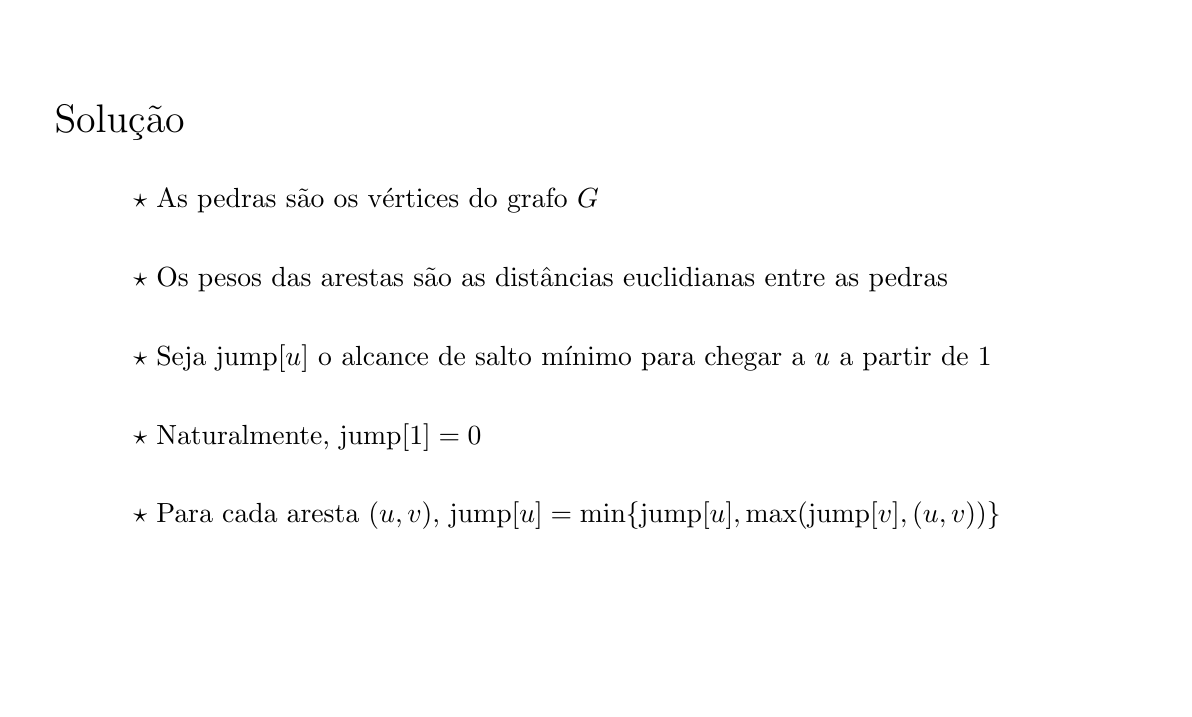
\begin{tikzpicture}
\node[draw,opacity=0] at (0, 0) {x};
\node[draw,opacity=0] at (14, 8) {x};
 \node[anchor=west] at (0, 7) { \Large \bbbold{Solução} };
 \node[anchor=west] at (1, 6) { $\star$ \bbtext{As pedras são os vértices do grafo $G$} };
 \node[anchor=west] at (1, 5) { $\star$ \bbtext{Os pesos das arestas são as distâncias euclidianas entre as pedras} };
 \node[anchor=west] at (1, 4) { $\star$ \bbtext{Seja $\mathrm{jump}[u]$ o alcance de salto mínimo para chegar a $u$ a partir de $1$} };
 \node[anchor=west] at (1, 3) { $\star$ \bbtext{Naturalmente, $\mathrm{jump}[1] = 0$ } };
 \node[anchor=west] at (1, 2) { $\star$ \bbtext{Para cada aresta $(u, v)$, $\mathrm{jump}[u] = \min\{\mathrm{jump}[u], \max(\mathrm{jump}[v], \dist(u, v))\}$ } };
\end{tikzpicture}
\end{frame}

\begin{frame}[plain,t]
 \inputsnippet{cpp}{9}{28}{codes/534.cpp}
\end{frame}

\end{document}
